\chapter{Comparative result \& experimentation on waypoints positioning } 
\minitoc
To remind, the main objective is to propose an efficient path to can cover an area using a camera mounted on an UAV. The solution proposed here, is to focus on optimizing the position of a cameras set to fully cover an area in a first time. When set of optimized cameras pose is found the position can be used as waypoints for an UAVs path. Indeed find an optimized position for each camera of a given set is primordial. The following sections are dedicated to the optimization of it. 




%\section{An optimization problem.}



\section{ Waypoint  positioning context of experiments} \label{sec:contextOfExp}

 During the previous sections, the problem was discussed as an optimization problem. The formulation of the problem was presented and also the complexity of the problems was discussed in the section \ref{sec:OptimizationComplexity}. 
The precedent sections has introduce all the useful elements to solve the problems of camera positioning in a complex environment. 
This chapter is dedicate to the different experimentations done to test the efficiency of the proposed methods. 
For the first experiment, different environment are proposed. The parameter of the environment has been adapted and chosen carefully. 
The environment have been designed to have a different shape and size. The different rooms shape are used to estimate the impact of the shape on the proposed solution.
The shapes of the rooms are designed to estimate the exact number of cameras in order to have a ground trough.
Moreover the rooms propose different size. The size of the room may have two main impact on the optimization.
First, increase the size of a room, will increase in proportion the size of the search space. On the other hand a bigger room allow to place more waypoints. More the number of waypoints to place is important more the number of dimension raise-up. The increasing number of dimension is used to test the robustness of the algorithms.
 The room finally used for the experimentation are proposed in the \figref{fig:Rooms_shapes}.
 
 \begin{mfigures}[!]{For the experiments: (a), (b), (c) the blue rectangle represents the field of view of one camera projected onto the ground  with z=1 ($30 \times 20 $px) and (d), (e) with z=2 ($60 \times 40 $px)}{fig:Rooms_shapes} \centering
\mfigure{width=.4\linewidth}{img/fig7-a.png}{Simple room}{subfig:r1}
\hspace{1cm}
\mfigure{width=.4\linewidth}{img/fig7-b.png}{Big room}{subfig:r2}
\mfigure{width=.4\linewidth}{img/fig7-c.png}{Room U}{subfig:r3}
\hspace{1cm}
\mfigure{width=.4\linewidth}{img/fig7-d.png}{Room L}{subfig:r4}
\mfigure{width=.4\linewidth}{img/fig7-e2.png}{Big room L}{subfig:r5}
\end{mfigures} 


% Due to the use of a non heuristic algorithms the shape can be considered as complex. The rooms are depicted in Figure \figref{fig:Rooms_shapes}, with areas of different size and shapes, where:  ...  
%,


%Thanks to this preliminary result the following section is only focused on the optimization process. 

\section{Other algorithm used}

In order to compare our proposed method other algorithm  has to be introduce. The following section will show the 2 algorithms used for the comparison to the proposed GA. The environment introduce in \ref{sec:contextOfExp} is used to  make this comparison.  
The particle swarm optimisation and the random selection is described in the following section. These two  algorithms was used due importance in the literature for the PSO and the other for this simplicity for evaluate the optimization.  

\subsection{PSO }

The PSO (Particle Swarm Optimization) is an algorithm dedicated to the optimization problems. It is a stochastic algorithms from the family of evolutionary algorithms (see chapter \ref{chap:EA}). 
The PSO is a relatively young compared then the other EA. It was developed by Russel Eberhart and James Kennedy in 1995 [148* bis]\cite{148*eberhart1995}. The concept of PSO is to optimize iteratively a continuous non linear function. To do that the PSO is inspired by the behaviour of animals. As it appends here from the bird flocking, fish schooling and swarming theory. These are animals working in a group to seek food. 
The direction to take is not decided by one leader, but by all individuals in the swarm by relaying just few informations as what quantities of food they found. 
The swarm composed by numerous individuals became smarter and more efficient to reach their objective. 
The algorithm proposed by Russel Eberhart and James Kennedy in [148* bis] \cite{148*eberhart1995} are directly inspired by these behaviours.

The methodologies used, is to examine each individual or also called particles as a solution of the problems. The problem is optimized at each iteration. To do that each solution must be comparable and quantifiable. At each iteration, each particle has to be tested by a cost function in order to discriminate the best particles of the swarm. The cost function and the design of it has been detailed in the chapter \ref{chap:formulation}.
When the best particle is found at the end of an iteration, the other particles of set, try to change their initial direction to converge more or less quickly to the actual best. 
Indeed the power of this algorithm is to obtain a very basic individuals behaviour to guide the particles. 
Each particle is guided by 3 behaviours.
 \begin{itemize}
 \item  This own velocity $V_k$. 
 \item  This own best solution $P_i$.
 \item  The best solution $P_g$.
\end{itemize}  
Here the velocity represents the useful speed of the particle to converge to the best solution. More the velocity is high more the step at each iteration will be long. 
The behaviour of the particles $X_k$ are modelled by the following equation to obtain the new position $X_{k+1}$ :
\begin{equation} \label{eq:PSO}
\begin{split}
 V_{k+1}= \omega V_k +b1(P_i -X_k)+b2(P_g-X_k)
\\
\mbox{ and } \\ X_{k+1}=X_k+V_{k+1}
\end{split}
\end{equation}

Where $\omega$ is the inertia. $b1$ is random value between 0 and $\phi_p$ and $b2$ is random value between 0 and $\phi_g$. $\phi_g$ and $\phi_p$  are the scaling factor to search away from the particles is best known position (Default: 0.5). 

Thanks to this basic behaviour of the particles the swarm can coverage to a global solution. 
To have an efficient optimization just few parameters must be set-up for the PSO.  
The more important are the inertia of the particles, the size of the swarm and the initial dispersion.
\begin{itemize}
\item The inertia will globally help the particles to keep their initial velocity. The consequences of the high inertia, is to explore more the search space and therefore the convergence will be longer. 
\item The size of the swarm  have an impact on the convergence time (in number of iteration) and  also the time computation. Indeed a big amount of particles in the swarm  means more exploration of the search space at each iteration, but also more comparison to find the best particles (the comparison may have a non negligible computation time). 
The swarm size is commonly fixed but can be as the population in the GA (see section \ref{sec:Population} ) dynamically adjusted during the optimization process. 

\item The initial dispersion of the swarm can be a decisive element as the population for the GA (see in \ref{sec:initPOP}). For the PSO the use of an heuristic to initialize all the particles of the swarm is not recommended due to this important risk to converge prematurely in a local minimum. The random dispersion appear as the more appropriate for a global optimization. On the other hand the fast convergence and the PSO ability to climb the small hill to go out of the local minima can be used in order to refine an other optimized solution. The principal risk is to optimize around the initial dispersion and do not explore correctly the search space.  
\item Other criteria as $\phi_g$ and $\phi_i$ are minor but can be useful to have a realy fine adjusted PSO.
\end{itemize}

Finally to summarize the PSO is efficient in term of optimization despite a very basic behaviour of each  particles. Each particle has this own velocity defined part way by the random and controlled by a global parameter; the inertia.
 The power of PSO is at the same time this efficiency to solve the optimization problem and this simplicity of use. In fact, the PSO needs at minima few element to work properly:
 A cost function, an inertia parameter and the size of the swarm. These efficiency and simplicity of use explain this popularity during the last decade.
 





%-the initial dispersion of the particles \\
%- size swarm \\
%- stopping criteria \\
%- inconvenient 


\subsection{Random selection }

The random selection (named RS) is a very basic algorithm. It serves as a reference points for the comparison of different algorithms. The RS does not take a complex meta-heuristic and is perfect to compare the efficiency of the other algorithm.

The random selection works by randomly generate numerous solutions. Among the solutions randomly generated the best solution is kept as the optimized global solution. The RS allows to look through the search space by randomly try different possible solution. The search space exploration by the RS is only made by random sampling without other optimization method. 
Indeed the RS is invoked as a reference points for the other algorithms. If the RS get a similar result with the same numbers of the cost function call, the algorithm compared can be considered as not more efficient then a simple random solution. 
The RS objective is to serve as  reference point for the other optimization algorithms. It will be a perfect reference to judge the efficiency of the optimization from other algorithms.  
  
%
%PSO camera position 
%8 33 87 84 143(transitor) 193 194 200(capter 360)201
%148 origine de PSO. 
%PSO[84 8 33 143] 87 193* 194* 200* 201* 
%
%228*(hibrid) 161* 158* 78 GA VS PSO

\section{Algorithm comparison }\label{sec:GAvsPSO} 
%
To solve the problem of cameras positioning (or waypoints positioning) the usable algorithms are varied as that was discussed in the chapter \ref{chap:stateOfTheArt} (see the sum-up tables \ref{tab:sum-up1} and \ref{tab:sum-up2}).
Among the algorithms studied in the literature the EA family appear as the more suitable to have an appropriate answer despite the numerous constraints of our problem. The EA is a vast family of algorithms. Among this family the more used for our problem is the PSO (see \ref{tab:sum-up2}). The PSO gives a good and fast result in many case. In the EA family, the GA is one of the founders and was one of the more popular due to this great flexibility and efficiency.
 After more investigation the GA is under estimate for the problem of camera positioning unlike the PSO (see \citep{33*reddy2012,8*zhou2011,84*xu2011,143*maji2015,193*fu2014,194*fu2010}).
 Base on the work of Boeringer et al in \citep{78*boeringer2004}, where the PSO and the GA have been conscientiously compared. The conclusions  of the comparison in \citep{78*boeringer2004} is relatively open and highlights the similarity of result between the two algorithms. An experimentation has to be done to find the best algorithms for the problem of cameras position in a complex environments. 



%The PSO and GA have been compared 
%The GA 
%158* 161* = GA PSO mimetic  conclusion les GA est plus long  le mimetic et  une solution intermedaire entre GA et PSO.
%78*= Comparaison entre PSO et algo génétique GA  les avantage  et les cas d’utilisation pratique.
%Papyer détatille  avec des plusier experience comparative  conclusion ouverte sur le choix mais la conlution et que le PSO offre plus de posibilité d’amélioration de par sa simplicité de mise en place et sa « récente utilisation » 

\subsection{Design of experiment }\label{sec:DoE}

%--------to finish-----\\ (+ integration du RS)\\

To find the best coverage, many experiments have been used to compare PSO and GA. PSO is easier to implement and runs faster, but GA is more flexible and generic thanks to the many tunable parameters. 
The following subsections will provide a comparison between PSO and GA with using RS as a reference.% and give an overview of our method, which is based on GA. The comparison demonstrates the overall advantage of the latter over the former.\\
%In the literature, the PSO was often used \cite{8*zhou2011,33*reddy2012}, mostly because of the simplicity of its implementation. However, it is interesting to compare the algorithm with the GA. The two algorithms are from the same family (both are stochastic and from evolutionary algorithms).\\
To compare and evaluate their performance, we tested them in different scenarios.

-!- The scenarios have been  designed to have a different shape and size. The shapes of the room have been designed to estimate the exact number of cameras in order to have a ground trough. Due to the use of a non heuristic algorithms the shape can be considered as complex. The rooms are depicted in Figure \figref{fig:Rooms_shapes}, with areas of different size and shapes, where: 




\begin{itemize}
\item[-]    z is the height of the camera between (within the range $[1/z;z]$).
\item[-]	Figure \figref{subfig:r1} is an area of size 120$\times$80 (named Room). 
\item[-]	Figure \figref{subfig:r2} is an area of size 240$\times$160 (named Big Room).
\item[-]	Figure \figref{subfig:r3} is an area of size 120$\times$80 (named Room U).
\item[-]	Figure \figref{subfig:r4} is an area of size 120$\times$80 (named Room L).
\item[-]	Figure \figref{subfig:r5} is an area of size 240$\times$80 (named Big Room L).
\end{itemize}


The design of the experiments in Table \ref{table:table1} has been set up to identify the most efficient algorithm for the positioning of a set of cameras with maximum coverage depending on the numerous cases. 
The Design of Experiments (DOE) has been made to take in account; the  shapes, sizes, some constraint as the fix altitude and  many size for the set of waypoints. The DOE has been established to highlight the impact of the constraints on the optimization process with the GA and PSO.


\begin{table} [!htb]
\begin{tabular}{|l|l|l|l|l|l|l|l|l|l|}
  \hline
  \multicolumn{2}{|l|}{ \Emph{z=1} } &\multicolumn{2}{|c|}{\Emph{GA}}  & \multicolumn{2}{|c|}{\Emph{PSO}} & \multicolumn{2}{|c|}{\Emph{RS}}  \\  \hline
  \multicolumn{2}{|c|}{ } & \textbf{GT} & \textbf{NC} & \textbf{GT} & \textbf{NC} & \textbf{GT} & \textbf{NC} \\ \hline
  \Emph{Room} &  \textbf{120x80} & 16 &20 & 16 & 20 & 16 & 20\\ \cline{2-8}
     &  \textbf{240x160} & 64 &70 & 64 & 70 & 64 & 70 \\ \hline
  \Emph{Room U} &  \textbf{120x80} & 12 &20 & 12 & 20 & 12 & 20\\ \hline
  \multicolumn{2}{|l|}{\Emph{z=2} } &\multicolumn{2}{|c|}{\Emph{GA}}  & \multicolumn{2}{|c|}{\Emph{PSO}}& \multicolumn{2}{|c|}{\Emph{RS}}  \\  \hline
  \multicolumn{2}{|c|}{ } & \textbf{GT} & \textbf{NC} & \textbf{GT} & \textbf{NC} & \textbf{GT} & \textbf{NC} \\ \hline
 \Emph{Room} &  \textbf{120x80} & 4 &10 & 4 & 10 & 4 & 10\\ \cline{2-8}
     &  \textbf{240x160} & 16 &20 & 16 & 20 & 16 & 20 \\ \hline
 \Emph{Room L}&  \textbf{120x80} & 3 &10 & 3 & 10 & 3 & 10\\ \cline{2-8}
     &  \textbf{240x160} & 15 &20 & 15 & 20 & 15 & 20 \\ \hline
  
\end{tabular}
\caption{Design of the experiment for comparing the efficiency of PSO and GA in different conditions.  (GT is Ground Truth and NW is Number of Waypoints).}\label{table:table1}

\end{table}

The Ground Truth (GT) is the minimum number of cameras required to fully cover a given area. The size of the area has been selected so that the GT can be easily estimated. 
NW is the maximum Number of Waypoints (or cameras) used for the experiments.  
At each experiment a solution is computed for a number of cameras from 1 to NW. To compare the different algorithms fairly, only 10 000 calls of the cost function are allowed for each optimization.
The optimization has been executed 8 times for each optimization process. 8 times is the minimum number of test has to be done to can have a usable average despite the hight volatility due to the randomness of the algorithms.\\ % 420*8 =3 360 test.


\subsection{ Analysis of the result }

\begin{figure}[!]
\minipage{0.99\textwidth}
  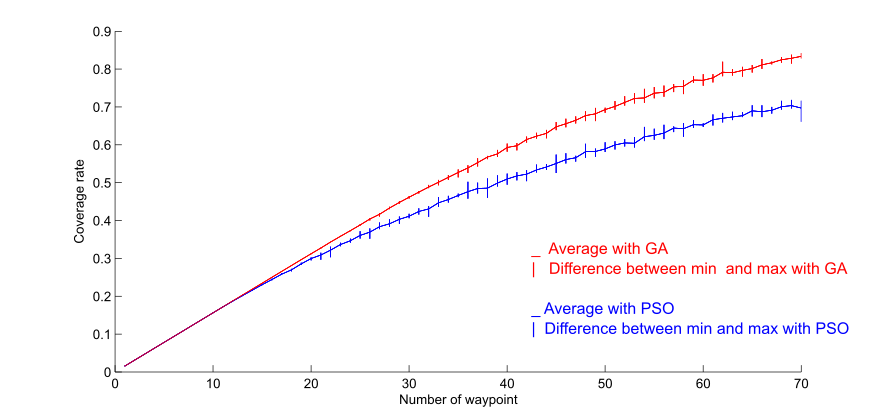
\includegraphics[width=\linewidth]{img/fig8.png}
  \caption{ Comparison of eight solutions given by the GA, with eight solutions given by PSO algorithms with a fixed altitude ($z$ equal to 1) in the big room $240\times160$. The ground truth for this room equals to 64.}
  \label{fig:bigRz1}
   \endminipage\hfill
\end{figure}
%
%
\begin{figure}[!]
\minipage{0.99\textwidth}
  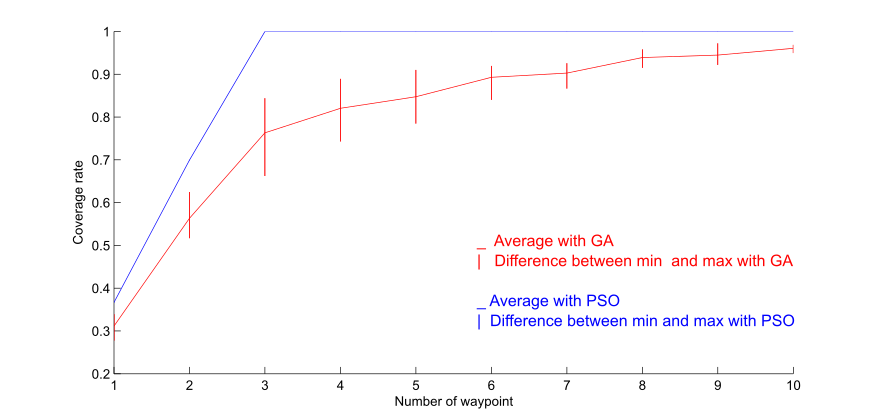
\includegraphics[width=\linewidth]{img/fig9.png}
  \caption{Comparison of eight solutions given by the GA, with eight solutions given by PSO algorithms with a Z between $[1/2; 2]$ in the room with L shape $120\times80$ and ground truth equal to 15.}\label{fig:RLz2}
   \endminipage\hfill
\end{figure}
After performing several experiments (see Table \ref{table:table1}), it appears that the GA and PSO algorithms are close in performance in numerous case. Among several experiment of the DoE some particularity appear despite the globally close result of GA and PSO. Also as expected the RS is always the worst solution.
 In the following subsection just few experiments are taken to illustrate some interesting phenomena specific to the GA and PSO for our problems.

In the case where the search space is large and numerous dimension have to be optimized by the GA appears globally more efficient as in Figure \ref{fig:bigRz1}. In contrary in this case (big room with z=1) the PSO gives a very bad answer close than simple RS.
%What is appearing in some case as in Figure \ref{fig:bigRz1} is the  GA is much more efficient where the search space is large (big room and big number of cameras),  as the example in Figure \ref{fig:bigRz1}. 
 Instead, PSO is more effective for optimizing small areas as in Figure \ref{fig:RLz2}. In the small room in L shape with a $z$ between 1/2 and 2, the PSO reach quickly (quicker than the 10 000 calls) to the optimal solution. Where, here the optimal solution is known and equal to GT. In the same case the GA propose an optimized solution (compared then the RS) but far from the PSO.
 
 This efficiency can be explained by the slight variation of the solution introduced by the PSO. However, this slight variation is not enough to find an optimized solution in a big search space that occurs when many cameras are required or when the local minimum is deeper. The PSO appears really efficient in a relatively small search space where the number of dimensions to optimize is not too high.
 On the other hand, the variety  introduced by the GA allows to escape from  the local minima. This variety is helpfully  in the big search space in order to explore quickly a wide part of it. The variety introduced by the GA became a handicap for a more fine optimization. That explains the bad result obtained during the experiment in the small room. The variety of the GA negatively affects the accuracy of the solution and may require a further optimization step to refine. 
 
%-------- ajouté un exemple entre 2 forme differente qui on un resulta proche ------------ file Grafig roomShape.txt-----\\
%The DoE have been design with different shape in order to see the impact of it on the algorithms. What is appearing during the experiment is the low impact of the shape on the result of the algorithms. The experiment made in the small room (120X80) and the small room in L shape with a z between [1/2; 2](see Figure !!! and Figure !!!). The graphics (see Figure !!! and Figure !!!)  present a similar result, proof of the small impact of the shape on the algorithms.
% This small impact can be explained by the use of meta-heuristic (as PSO and GA) and not by the use of an heuristic  much more dependent of the shape (and the constraint). 
% 
%Thanks to that we know the two algorithms can be used for a more complex shape as that will be presented in the following experiment.

 





% Following the comparison of the 2 algorithms, the GA seems more suited for finding UAV waypoints especially if it navigates in a large room or  outdoor scenes.
%Furthermore, our comparative study demonstrates that the GA is less dependent on the shape of the area to cover. \\
%------------------
%According to the previous results, the genetic algorithm will be used during future work with no restriction at the convergence point to optimize the positioning of the waypoints in the bigger areas seen in Section  \ref{coverageOutDoor} such as in Figure \ref{subfig:satimg+mask}.\\
%---------------

%fill with the jirs 
%	\subsection{DoF Design of Experiment}
%	\subsection{Result}
%	\subsection{Explication}

\section{Hybrid GA PSO }\label{sec:hybridGAPSO}
% ref: 76* 77* 
 

% l'hybridration peut permetre de tiré avantage des 2 algo
% \begin{itemize}
%  \item interer de l'hybridation (avantage du PSO sur l'optimisation locale et du GA) 
% \item les forme d'ibridation possible 
% \item la plus aproprier dans notre cas et pourquoi 
% \item les experience ( the experimentation  was done in the Big room in L shape as the \ref{fig:Rooms_shapes}.e)
% \item les resultats
% \end{itemize}
Thanks to the experiment done and presented in the previous section (see \ref{sec:GAvsPSO}) the GA and PSO are two algorithms efficient and complementary to solve the problem of camera positioning in the complex and potentially vast area.
  To summarize the preceding comparison, it is difficult to rank the two algorithms in all the environments. GA and PSO have both advantages depending on the area and the number of waypoints to pose estimate. GA is better in the vast search space and for several dimension to optimize. When PSO is efficient to refined faster the solution.
 The hybridization can be the key to optimize the camera positions in all the condition. The aim of the hybridization is to exploit the better of both algorithms, trying to further refine the solution. 

%   77*\cite{c13}.
\subsection{The different hybridization }

 Different hybridization of the GA and PSO can be made. Each hybridization of GA and PSO has the advantage and disadvantage. This following section is focused on the main hybridisation of GA and PSO. \\
In Premalatha al et 76* \citep{76*premalatha2009} propose three different solution to hybrid the GA and PSO: 
\begin{itemize}
\item  GA and the PSO are employed in parallel. The best solution between both algorithms is used into the other algorithm. 
For example: If the best solution at the end of the first generation is from PSO, this solution is used as a new individual for the crossover on the GA. Or if the best solution is from the GA, this good individual is employed in PSO as best particle for the next draw. This operation continues until such time as the convergence of both algorithms.   
%(LA MEILLEURE SOLUTION DES DEUX EST INJECTEE DANS L'AUTRE : CA VEUT DIRE QUOI ? ET TEL QUE DECRIT, CE N'EST PAS DU PARALLELE ! MIEUX EXPLIQUER)
 
\item The GA is used to introduce variety on the PSO, when the PSO is stagnating. Stagnated states are reach when no solution upgrades after a predefined number of iteration. In this case, the GA introduces variety by proposing other solutions for PSO. This hybridization has to be managed carefully due to this high risk of non convergence. 

\item The GA is used until the convergence point. When the GA converge to a solution, the PSO is used to refine with one more optimization. This solution is costly in time due to this double optimization and this double convergence. Finally this hybridization uses the GA optimization as an initialization for the PSO.\\
\end{itemize}

The last hybridization, using GA as initialization for PSO is probably one of the most suitable for the problems of camera positioning in a vast and complex area. 
The experiment made until now (see \ref{sec:DoE}) confirm the mechanism described by the last hybridization of GAPSO. In fact for our problems GA is efficient to run through all the search space and in the other hand the  ability PSO to refine the solution is also confirmed.  
In this case, the GA can be a very good initial guess for the PSO. \\

In Shi et al \cite{77*shi2005} the hybrid PSO GA (same as GA and PSO employed in parallel) was studied for 6  problems listed F1 to F6. The 6 problems have a global optimal knew.  In this article \cite{77*shi2005} the different problems are used to demonstrate the efficiency of hybrid PSO GA and search the appropriate set up for their parameters. One of the interesting aspects presented in \cite{77*shi2005} is the importance given to find  the best set-up for each algorithms. 
The set-up of the algorithms has to be adapted to the hybridization and the problems. As that was disused in shi et al \cite{77*shi2005}  numerous tests have to be done to find it.

 In our case, the GAPSO is used within a first time a GA and a PSO next to refine the solution. In this case, the GA has to introduce even more variety in order to be more efficient. Consequently the GA has to be modified to have a mutation ratio higher.   



\subsection{Experimentation }
To compare the efficiency of the hybridization GAPSO to the GA, one experimentation is proposed.
The experimentation followed the rule fixed during the comparison as in Table \ref{table:table1}. %\\
It appears the big room in L shape as the Figure \figref{subfig:r5} is the most suitable to test the hybridization.  % (POURQUOI ???).
The L shape room proposes a big search space which can require a big amount of cameras to cover it. This configuration is the most likely to be improved on a different situation, also closer to a realistic configuration.\\
The proposed experiment uses the GA for a maximum of 100 generations and the GA solution as an initialization for the PSO. Also the PSO is locked at 100 iterations. %(C'EST L'EXPERIMENTATION QUI PROPOSE ?). \\%Finally the GAPSO are used for an amount around 20000 call of the cost function or the GA use onnly 10000call but the result of GA wiht 20 000 call are similaire then the 10000 (show fig). like that the encreasing is due to the hibridization and not to the morte time computation allowed. 

The set-up of the GA has been slightly modified by increasing the mutation ratio and the PSO is also adapted by reduce the inertia.
 Before to reduce the inertia of the PSO few test was quickly made, especially with a dynamic inertia. A dynamic inertia can be efficient and allow the PSO to start with a bigger inertia to visit more the search space at the beginning and time after time the reduction of it help the PSO to converge faster. In this case, a small decrement of the inertia is applied at each iteration. Finally this method does not provide a significant gain. The dynamic inertia is finally  not really useful in the context of hybrid GAPSO. The solution  preferred for the PSO set-up has a slightly lower inertia parameter (around 0.4).

\begin{figure}[t]
\minipage{0.85\textwidth}
  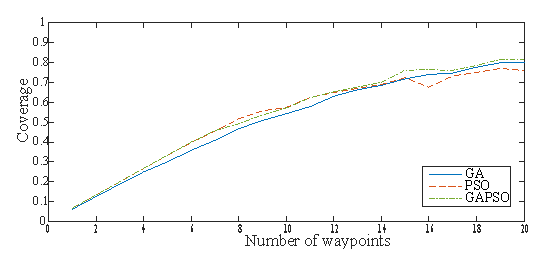
\includegraphics[width=\linewidth]{img/GAPSO_GA_PSO3waypoint.eps}
  \caption{comparison between GA PSO and the hybridization of GAPSO.
}\label{fig:GAPSO}
  \endminipage\hfill
\end{figure}

 \subsection{Result and comment }
  
%\begin{figure}[t]
%\minipage{0.95\textwidth}
%  \includegraphics[width=\linewidth]{HibridLroomGAPSO2.png}
%  \caption{GA vs GAPSO.
%}\label{fig:GAPSO}
%  \endminipage\hfill
%\end{figure}

The big room in L shape where the comparison between simple GA and PSO was performed, is also used to compare the GAPSO efficiency. The GAPSO is compared with the single GA in one side and the single PSO on the other side. 

In the Figure \ref{fig:GAPSO} it is appearing the hybridization of GA, PSO increases slightly the percentage of coverage.%(around 0.0002 and 0.107 point of percentage)
This graphic can be split in 2 parts, the left side with a relatively low number of waypoints (or cameras) to pose estimate (until 15) and the right part with more waypoints. To remember in this experiment for each camera (or waypoint) is defined in x, y and z. That means for 15 waypoints, 45 dimensions have to be optimized.
The two sides of the graphic show efficiency of the different algorithms and confirmed the mechanism of GA and PSO.
The PSO is more efficient in the beginning when the numbers of dimensions to optimize are reduced. Otherwise as we saw previously the GA is efficient in the big search space with an important amount of dimension to optimize. The GA became better than the PSO in the right part of the graphic \ref{fig:GAPSO}. 
The solution  proposed by the GAPSO on the left side of the graphic \ref{fig:GAPSO} is equal or a bite better then the PSO. On the other side, the GAPSO propose a solution more refine than the simple GA. This refinement is due to the PSO ability to optimize the solution from the first optimization (GA). 

Finally the biggest advantage of the GAPSO is to propose most of the time the best solution and some time slightly better by combining the advantage of both algorithms. 
The GAPSO can reduce the limitation of the GA and help to go deeper in the optimization process. The GAPSO  beside to upgrade the solution initially proposed by a simple GA or PSO offer more flexibility and allow only one solution to be efficient. The GAPSO is efficient despite the number of dimensions to optimize and potentially more robust depending on the size of the search space.
Despite these great advantage (better solution and more flexibility).
The principal inconvenient of the GAPSO is caused by this double convergence. In fact with a hybrid GAPSO, as we decide to use a GA has to be executed until a convergence and in the second time optimized with a PSO. Obviously this implementation increases the time of computation.
 
   
% This refinement is due to the PSO ability to optimize the local solution. As we saw previously the GA is efficient in the big search space and with a big amount of dimension to optimize, but the solution gives the GA need some local adjustment to be better. The GA has few limitation to go deeper in the optimization process but this weakness is partially corrected by the hybridization. The principal advantage hybridization is the ability to keep the benefit of both algorithms. The Figure \ref{fig:GAPSO} show that the GAPSO proposes most of the time the best solution or equal to the best solution by combining the advantage of both algorithms. 
%	\subsection{memetic ???}
%		\subsubsection{DoF}
%		\subsubsection{Result}
%		\subsubsection{Conclusion}
		
\section{Going further, more experiment }

The previous section with the different experiments shown the efficiency of the GA for the vast areas and the flexibility offer by the hybridised GAPSO (with a small refinement of the solution). The experiments made until know was focused on different area relatively simple the next step is to increase the difficulty of the scene. The increased complexity is made by adding: 
\begin{itemize}
\item More obstacle.
\item Hole in the area.
\item Increase size of the area.
\item Increase the search space by adding more parameters(as the roll). 
%\item Add new constraint (as  some fix cameras).
\end{itemize} 
The following section present the results obtained by increase step by step the difficulty. Each step presented chronologically in the following section has been made to test and some time to refine the parameters of the GA and GAPSO in different contexts. In the following section only the more significant step has been presented.

	\subsection{Rectangle obstacle } \label{sec:expRectObstacle}
	\begin{mfigures}[!]{Indoor area coverage using V-rep to simulate a realistic environment.}{fig:RoomsVrep} \centering
\mfigure{width=.4\linewidth}{img/room_full.png}{Room in V-rep.}{subfig:VrepRoom}
\hspace{1cm}
\mfigure{width=.4\linewidth}{img/room_python.PNG}{Poses of every image captured in the room.}{subfig:WaypointPoseVrep}
\mfigure{width=.4\linewidth}{img/mosaic2.png}{Reconstructed room based on the waypoints positions.}{subfig:mosaicSceneVrep}
\hspace{1cm}

\tabsimuposeVrep
\end{mfigures}
	
	Thanks to the result obtained (see \ref{sec:hybridGAPSO}) an experiment is made using a slightly bigger size than the big room (in Figure \figref{fig:Rooms_shapes}). The environment of this experiment to try to be more realistic, consequently the room is designed with more obstacle. 
	The obstacles are added in the map as non-interesting area to cover as explained in  section \ref{subPara:MapConstraintAndObstacle}. Also for the first time the design of this room  is  not made in order to have perfect ground trough unlike the previous room design (Figure \figref{fig:Rooms_shapes}). The consequence of it is the number of camera use to cover all the area is not an integer and some overlap must append.
	For this first realistic experiment a simulation tool dedicate to robotics is used to illustrate the result. 
	     
	The simulated room is 15 $\times$ 14 m$^2$ which corresponds more or less to a large lecture hall. The areas in red (see Figure \figref{subfig:VrepRoom})represent the zones which do not require coverage. Every camera can cover a 4 $\times$ 3 m$^2$,  when $z$ is equal to one. The $z$ factor can be equal at $[0.5, 1, 1.5]$, and the cameras can turn  at 90$^{\circ}$ to have the image in portrait or landscape. All of these parameters are taken into account in order to compute the waypoints position.The optimization of the waypoints position is made using  only the GA, but this time it is applied until the convergence. 
	
	 After running the single GA  a well optimized waypoints positioning is given (see Figure \figref{subfig:WaypointPoseVrep}). Not perfect but good enough with a limited number of cameras. At Each waypoints an image is captured in order to offer a  mosaic image of the scene with a restricted number of small black holes (see Figure \figref{subfig:mosaicSceneVrep}).
	  The solution obtained is comparable to the experiments made previously (see \ref{sec:DoE}). As aspect, despite the increasing number of obstacle and increased size of the search space. This confirms again the ability of adaptation of the EA optimization and more exactly the single GA. These results encourage us to go  further. 

%%%%%%%%%%%%%%%%%%% for the  path plan%%%%%%%%%%%%%%%%%%%%%%%%%%%%%%%%%
% refer to : https://en.wikipedia.org/wiki/Screw_theory#Twist

%These messages contain the linear and angular velocity values needed to control the robot's position and orientation. This process is to make the transition from simulation to real world UAV straightforward. The number of waypoints is set depending on the area covered by the cameras projection figure \ref{fig:cam_proj}. The trajectory built from these waypoints is done by sub-sampling the space between these 3D points coordinates.\\
%In our experiments, V-REP \cite{Vrep} is used to simulate the hardware of the UAV and all its mounted sensors like camera which is the core sensor. 
%% It was also used to build the room as explained in more details in the next subsection (\ref{experiment}). 
%In order to ease the deployment of the algorithms on a real platform, we chose ROS \cite{ROS} as the implementation framework to command the simulated UAV.
% This experiment follow the pipeline showed in the figure \ref{fig:pipeline} with the two different optimization parts.\\
 




	\subsection{Rectangle obstacles with hole}\label{sec:RecObstacleHole}
%	C:\Users\stru\Documents\python\hold on\satelit Imag
%	C:\Users\stru\Documents\python\Complex room\sat LEII

%	C:\Users\stru\Documents\python\hold on\map 120 to compute\cam40X40 minNmbCamCover100=98cam exec 1h
%	C:\Users\stru\Documents\python\satelite img\barrientosMap
%	C:\Users\stru\Documents\python\camfix 	
\begin{mfigures}[!]
{Coverage area from satellite images with 75 cameras for a coverage of $76.39\%$ using the the GA.}{fig:Le2iCubeMap} \centering
\mfigure{width=.4\linewidth}{img/LE2Imap.png}{The area to cover taken form satellite images.}{subfig:Le2iCube}
\hspace{1cm}
\mfigure{width=.4\linewidth}{img/EmptyCubRoom.png}{The mask of the area to cover.}{subfig:satimgMask}
\mfigure{width=.4\linewidth}{img/LE2I_GAevolvTurnComplex76_47481899.png}{Area cover by the network of cameras using the GA.}{subfig:IUTCoverage}
\hspace{1cm}
\tabsimuposeIUTcube
\end{mfigures}	

The previous experiment shown the efficiency of the single GA despite numerous obstacle and slightly bigger room. The following experiment try to push a bit more the optimization process using a single GA. The increased complexity of map was made by adding much more obstacle with some holes in the middle of the map. In fact until know all the obstacles was added around the bounding of the area. Add Obstacle in the middle to create a hole in the area, that increase significantly the complexity of the coverage estimation.
To simulate a realistic environment the map is designed manually based on a satellite images (see Figure \figref{subfig:Le2iCube}). Each rectangle obstacle has been placed to reproduce the buildings as in  the satellite images. 

The result obtained by the GA optimization (see Figure \figref{subfig:IUTCoverage}) show one more time the adaptation power of the single GA to the complex scene. The total coverage of the area is around $76.5\%$ for 75 waypoints. The answer proposed is not perfect and can be improved in order to reduce some overlap and black hole. The important number of dimension to optimize ($75\time 4$) and the increased size of the area (twice bigger then previously) mark the limit of the simple GA optimization.\\
	The more interesting aspect of this experiment is to show the efficiency of the single GA in a real complex environment. The solution proposed can be considered as good for the purpose of the challenge (obstacle, hole, numerous waypoints to pose estimate, vast area,...). 
  
%only GA 
%z size  0.5 1 1.5 1.75
%waypoint snap
%camera size 31x24 px

	
	\subsection{Using mask to describe the area }\label{sec:maskGAPSO}

\begin{mfigures}[!]
{Coverage area from satellite images with 25 cameras for $90.76\%$ of coverage using the GA and $92.81\%$ of coverage using the GAPSO.}{fig:TorcyMap} \centering
\mfigure{width=.4\linewidth}{img/torcy3.png}{The area to cover taken form satellite images.}{subfig:satimgTorcy}
\hspace{1cm}
\mfigure{width=.4\linewidth}{img/torcy4.png}{The mask of the area to cover.}{subfig:satimgMaskTorcy}
\mfigure{width=.4\linewidth}{img/Torcyz90GANcam25.png}{Area cover by the network of cameras using the GA $90.76\%$.}{subfig:coverageGATorcy}
\hspace{1cm}
\mfigure{width=.4\linewidth}{img/TorcyGAPSO_hybridCout_92Ncam_25.png}{Area cover by the network of
cameras using the GAPSO $92.81\%$.}{subfig:coverageGAPSOTorcy}
\tabsimuposeTorcy
\end{mfigures}


Based on the limitation of the map design and the necessity to go one step further the paradigm has to evolve.
The solution proposed representing the area until now, was to add rectangles obstacles by removing the corresponding points of the grid (as explained in \ref{subsec:obstacleZone}). The primary advantage to use rectangle obstacles was in the coding implementation. 
This facility becomes a lock for the more complex area. In addition, it is revealed not user friendly.\\
 The solution chosen for the flowing experimentation is to use a binary mask of the area to cover. The mask represents in the white side the area to cover and in  the black side of the non interesting zone (also called obstacles, see \figref{subfig:satimgMaskTorcy}). This solution is finally more "user friendly"  and do not change the fundamental of the grid map used until here. Each white pixel of the mask is a point of the grid to cover.  
 
%from VISAP EVOLUTIONRY ALGORITHM FOR POSITIONING CAMERAS NETWORKS MOUNTED ON UAV torcy map

For this first experiment with the binary mask to describe the area to cover, a smaller area is selected. A smaller area involved a smaller amount of similar waypoints necessary to fully cover it. In the Figure \figref{subfig:satimgTorcy} the area to control is extracted from a satellite images to have a mask (see\figref{subfig:satimgMaskTorcy}). The single GA is performed  with 25 waypoints to pose estimate. The solution obtained by the single GA is re-injected in the PSO. Each waypoint has to be placed on $x; y; z$. In order to test this new paradigm the rotation $\gamma$ is removed from the parameters to optimize.

 To begin the single GA was performed. The result are visible in Figure \figref{subfig:coverageGATorcy}. The optimized waypoints positioning, cover $90.76\%$ of the area with 25 cameras and the single GA converge after just 67 generations. The solution given by the single GA is already good enough despite the complexity of the map. 
  The solution obtained is conformed to the expected result. The solution of the single GA gives a well optimized waypoints poses, despite the new paradigm with the complex map. 
  
   Among the experiment presented until now (\ref{sec:RecObstacleHole} and \ref{sec:expRectObstacle}) only the single GA was employed for the optimization. On the last experiment (\ref{sec:RecObstacleHole}) with a bigger and more complex area composed by hole,  the limiting of a single GA appears slightly. This observation is confirmed and is getting bigger for the area more complex. More complex as the one outcome the map designed according to the satellite images with mask (as  Figure \figref{subfig:satimgTorcy} and \figref{subfig:satimgMaskTorcy}).
The solution proposed being to apply a GAPSO. The PSO will allow the refinement of the GA solution.
%Consequently, the GA is performed  firstly to optimize the position of the waypoints . 
%The optimized waypoints positioning, cover $90.76\%$ of the area with 25 cameras and the GA converge after just 67 generation. The solution given by the single GA is already good enough despise the complexity of the map. Although can be refined by apply a PSO. 
The PSO is used with an initialisation from the first optimisation (using  the GA solution). 
Finally the result presented in the Figure \figref{subfig:coverageGAPSOTorcy} shown a much more refined  coverage with significant reduction in the amount of black hole and overlap (coverage is over $92.8\%$). 

The main result of this experiment was to evaluate if the paradigm modification may have a significant impact on the waypoints positioning.
 The conclusion of this experiment is, in fact not so much when the GAPSO is applied. Despite the increased complexity due to the area shape (possible by the mask) the use of the hybrid GAPSO permit to composentes it. The experiment allows also to evaluate the improvement made by the GAPSO. The GAPSO hybridization is robust and flexible despite the strong constraint due to the non geometric area.  

Thanks to this tries the size of the area to cover and the number of waypoints can be increased. The next experiment has to test the boundary of the GAPSO optimization in term of size and number of cameras using a mask for describing the area.


	\subsection{Using mask for bigger area}
	Based on the last experiment (\ref{sec:maskGAPSO}) a much bigger area with much more waypoints to pose estimates are presented here. The goal of the following sections is to see the boundary of the  GAPSO optimization when the sliders are pushed to the maximum. The maximum in term of area size, number of waypoint and shape complexity.
	
		\subsubsection{Vast and complex outdoor}\label{sec:fey_map}

\begin{mfigures}[!]{ Optimization of the waypoints poses with a vast outside area and just a few  black holes.}{fig:Rooms_shapes} \centering
\mfigure{width=.4\linewidth}{img/fig12-a2.png}{The area to cover taken form satellite images.}{subfig:satimgFley}
\hspace{1cm}
\mfigure{width=.4\linewidth}{img/fig12-b2.png}{The mask of the area to cover.}{subfig:satimgMaskFley}
\mfigure{width=.4\linewidth}{img/fig12-c2.png}{The result of the coverage with the waypoints position.}{subfig:satimgcoverageFley}
\hspace{1cm}
\mfigure{width=.4\linewidth}{img/fig12-d4.png}{The final mosaic images}{subfig:satimgNoncoverFley}
\tabsimuposeFley
\end{mfigures}


In this experiment, a much bigger and complex area is presented.
		A much bigger area involves the increasing of the search space and consequently the increasing of the complexity. 
In the following example Figure \figref{subfig:satimgMaskFley} the satellite images are used to define the area to control (in white). The size of the area has been increased to have a grid composed by almost half million of points with nearly to 200 thousands points to cover. 
The objective is to increase the difficulty in this experiment. In addition to the increased size of the area to cover, the shape of it has been complicated. To do that an area with several sub-parts composed by small space and hole has been selected.\\
During this experimentation, a high coverage rate is required. We aspect more than $95\%$ of coverage rate. More than $95\%$ of coverage rate is a hight requirement and push the optimization in term of precise positioning to the limit of the GAPSO. The risk to ask a very hight coverage rate is to need a lot of waypoints with several overlap and consequently a long time before to converge. 
%File name :C:\Users\stru\Documents\python\newMap  champ\fley71390RMask.png
%Size is : 895 x 502
%Nmb point to cover: 194497
%Nmb point to non cover: 253397
%total:447894
%/!\ The image given is not a falide mask dif : -1396

In order to cover the big area, the solution can be to use a bigger focal length or higher altitude to have a wide area covered at each waypoint, thus keep few waypoints to control the area. The other solution is to increase the number of waypoints. The increased number of waypoints can be a source of difficulty for the  optimization. Although the difficulty to manage more waypoints  to the GAPSO associate to the adapted cost function allows the example Figure \figref{subfig:satimgcoverageFley} more waypoints to be placed and optimized. 
 In the Figure \figref{subfig:satimgcoverageFley} and \figref{subfig:satimgNoncoverFley} the area is covered by 80 waypoints for $98.48\%$ of coverage. To reach this coverage rate the GA convergence is achieved after 4'856 generations. The important number of necessary generation before the convergence of the GA and a similar  increasing time computation for the PSO, allow us to glimpse the limits of the GAPSO for the too big search space with numerous waypoints to pose estimate. Despite this potential future limitation the answer of the GAPSO is relatively fast and efficient.\\
 

		\subsubsection{Biggest map with numerous waypoints}
\begin{mfigures}[!]{ Optimization of the waypoint pose with a big outside area: (a) is the area to cover take form a satellite images,(b) is a mask of the area to cover, (c) is a result of the coverage with the waypoint position, (d) is the representation of the black hole.}{fig:CalvissonExp} \centering
\mfigure{width=.4\linewidth}{img/calvisson2+mask.png}{The area to cover taken form satellite images.}{subfig:satimgCalvisson}
\hspace{1cm}
\mfigure{width=.4\linewidth}{img/calvisson2mask.png}{The mask of the area to cover.}{subfig:satimgMaskCalvisson}
\mfigure{width=.4\linewidth}{img/zcalvisson2result1cout_98_260375_gen_170501_Ncam_110.png}{The result of the coverage with the waypoints position.}{subfig:satimgcoverageCalvisson}
\hspace{1cm}
\mfigure{width=.4\linewidth}{img/calvisson3cover.png}{The final mosaic images}{subfig:satimgNoncoverCalvisson}
\tabsimuposeCalvisson
\end{mfigures}	

The precedent experiment (see \ref{sec:fey_map}) shows the efficiency and flexibility of the GAPSO to the big map with lots of waypoint in a really complex area. Despite an important increasing time of computation the GAPSO can use to go even more further and try to touch the boundary.  

For this experiment, the area proposed here is the biggest never tested yet (among the one presented). The grid is composed of almost 1 million of points, with more than 616 thousands points to cover. The number of waypoints to cover this vast area, has been increased to reach the 110 waypoints. 
The number of waypoints to pose estimate, is the among more important compared to the literature for example, in \citep{8*zhou2011,33*reddy2012,82*chrysostomou2012,143*maji2015, 151*zhao2013, 152*wang2009, 165*jiang2010, 193*fu2014, 181*wang2017, 18*ding2012}. %, ,83*van2009   bug ?
The GAPSO is executed with success and the final coverage is over $98.26\%$.  
	
	 To reach this coverage rate the GA convergence is achieved after 170'501 generations. \\
	 The important number of generation before to reach the convergence with the GA in a first time, and  proceed to a PSO optimization for a second time reveals a long time computation before the final solution given by the GAPSO. 
	 That show at the same time the great efficiency of GAPSO to optimize the position for numerous waypoints in a big search space with proposing a really good answer. This great optimization is conditionally upon for an important time of convergence. This show the limit of the GAPSO due to the important number of generation and consequently important time computation (a few hours with a core i7).  
	 To nuanced the really important time useful to reach the double convergence (GA and PSO) the context of the experiment has to be highlighted. In Fact the area to cover is important but also the coverage rate respected is also an important factor because more this coverage rate is important more a fine tuning of the numerous parameters of the solution must be done.
	
	\subsection{Waypoints positioning limitation} 
	
Among numerous experiments done, the GAPSO appear as a good solution to optimize the position and orientation of numerous waypoints (or cameras) in a vast and complex map.
In the first time the GA appear efficient enough for the optimization in the big room but after more experimentation the single GA appears weak to finally refine the solution. The contribution of PSO was essential to have a more refine solution and also allow more flexibility especially when the number of waypoints is restricted. \\
During the differents experiment proposed some limitation appear. Among the limitation the more important is mostly the consequences of a high numbers of waypoints to have a high coverage rate.
 The size of the area and moreover the number of waypoints to pose estimate has an important impact on the time convergence of the GAPSO.  This time convergence increase even more when the number of waypoints is hight  for have a high coverage rate. \\
 To illustrate this phenomenon the a GAPSO ran on the last experiment (same map) but  with less waypoints(only 80). Consequently the coverage rate is also smaller around $85.5\%$ of coverage for  the 80 waypoints. In this condition, the number of generation for the GA before to converge are just around 200 generation.  This 200 generations for the GA and a similar number of iteration for the PSO appears as a huge difference between the $98.26\%$ of coverage of the 110 waypoints in 170'501 generations. This huge difference is due at the same time to the number of dimension to optimize and the fine refinement due to the high coverage rate.
 Thanks to these observations it is appearing the main limitation of the GAPSO is not the  big or complex area, but is mostly the high number of waypoints (or number of dimension to optimize ) and the high coverage rate with involved a fine refinement of each waypoints position. 
 

%%%%%%%%%%%%%%%%%%%%%%%%%%%%%%%%%%%%%%%%%%%%%%%%%%%%%%%%%%%%%%%%%%%%%%%%%%%


%\begin{mfigures}[!]{ Optimization of the waypoints poses with a vast outside area and just a few  black holes.}{fig:Rooms_shapes} \centering
%\mfigure{width=.4\linewidth}{img/fig12-a2.png}{The area to cover taken form satellite images.}{subfig:satimgFley}
%\hspace{1cm}
%\mfigure{width=.4\linewidth}{img/fig12-b2.png}{The mask of the area to cover.}{subfig:satimgMaskFley}
%\mfigure{width=.4\linewidth}{img/fig12-c2.png}{The result of the coverage with the waypoints position.}{subfig:satimgcoverageFley}
%\hspace{1cm}
%\mfigure{width=.4\linewidth}{img/fig12-d4.png}{The final mosaic images}{subfig:satimgNoncoverFley}
%\tabsimuposeFley
%\end{mfigures}


  
% \hspace*{\fill}\subfloat[][]{\tabsimupose} 
 
%!!!!!!!!!!!!!!!!!!!!!!!!!!!!!!!!!!!!!!!!!!!!!!!!!!!!!!!!!!!!!!!!!!!!!!
%As demonstrate before with the previous experimentation the GAPSO is robust for a big outdoor area with a non-convex shape. This experiment show one more time for a similar area in term of size (a bit slower) with  less cameras. The objective is to increase the difficulty  by adding  an more complex shape of the area to cover. To do that an area with several sub-parts composed by small space and hole has been selected.
%During this experimentation a high coverage rate is required (we aspect more than 95%) 
%
%In the following example, shown in Figure \figref{subfig:satimgFley}, the satellite images are used to denote the area to control (in white). \\
%
% However the GA associated with the adapted cost function allows  (as in Figure \figref{subfig:satimgcoverageFley}) many more waypoints to be placed and optimized in order to keep an acceptable image resolution of the area compared to the literature, for example, in \cite{8*,33*}. In Figure \figref{subfig:satimgcoverageFley} and \figref{subfig:satimgNoncoverFley}, the area is covered by 80 waypoints for a 98.48$\%$ coverage rate, with an average $z$ at 0.95 and  the GA convergence is achieved after 4856 generations before an PSO optimization. \\
%		


%%%%%%%%%%%%%%%%%%%%%%%%%%%%%%%%%%%%%%%%%%%%%%%%%%%%

 


